\documentclass[
  10pt,
  a0paper,
  portrait,
  margin=0mm,
  innermargin=15mm,
  blockverticalspace=0mm,
  colspace=0mm,
  subcolspace=0mm
]{tikzposter}

\usepackage{amsmath, amssymb}

% multiple affiliations
\usepackage{authblk}
% modern font package
%\usepackage{lmodern}

\newcommand{\mf}{\mathbf}
\newcommand{\lb}{\left(}
\newcommand{\rb}{\right)}

\newcommand{\bbG}{\mathbb{G}}
\newcommand{\bbI}{\mathbb{I}}

\newcommand{\vverh}{\vspace*{-0.05cm}}
\newcommand{\vniz}{\vspace{0.05cm}}

\makeatletter
\def\TP@titlegraphictotitledistance{1cm}
\settitle{\centering \color{titlefgcolor} \vbox{\@titlegraphic \\ [\TP@titlegraphictotitledistance] \bfseries \fontsize{1.75cm}{1.3cm} \selectfont \@title \par} \vspace*{1em} {\fontsize{1.4cm}{1cm}\selectfont \@author \par}} 
\makeatother

\title{\parbox{\linewidth}{ \centering First spectral moments of collision-induced rototranslational absorption band of CO$_2-$Ar pair:} \\
Classical theory with the use of \textit{ab initio} calculated anisotropic interactions}

\author[1, 3]{\underline{Daniil N. Chistikov}}
\author[1]{\underline{Artem A. Finenko}} 
\author[2]{Yulia N. Kalugina}
\author[1, 3]{Sergei E. Lokshtanov}
\author[1]{Sergey V. Petrov}
\author[3]{Andrey A. Vigasin}

\affil[1]{Department of Chemistry, Lomonosov Moscow State University, 1-3 Leninskie Gory, Moscow, 119991, Russia}
\affil[2]{Department of Optics and Spectroscopy, Tomsk State University, 36 Lenin av., Tomsk, 634050, Russia}
\affil[3]{Obukhov Institute of Atmospheric Physics RAS, 3 Pyzhevsky per., Moscow, 119017, Russia}

\usetheme{Simple}

\usetitlestyle[width = \linewidth, roundedcorners=5, linewidth=2pt,titletoblockverticalspace=0mm]{Default}
\usebackgroundstyle{Empty}

\begin{document}

\maketitle

\begin{columns}
\column{0.5}
\block[titleoffsety=40cm, bodyoffsety=6.5cm]{Introduction}{
\vspace*{-38cm}
Much attention is presently devoted to the study of dipole-forbidden molecular absorption caused by weak intermolecular interaction. This interest is significantly motivated by the need to refine the accuracy of climate models which are being developed for the planetary or exoplanetary atmospheres. Actual knowledge of binary absorption coefficients is still fragmentary (see e.g. [1]) and is thus fairly unsatisfactory in regard of great number of pairs potentially interesting for climate modeling. Experimental observation of the weak pressure-induced absorption is especially difficult in the far-infrared where the most important so-called rototranslational collision-induced absorption (RT CIA) bands are conventionally situated. Direct quantum calculations are still barely feasible for interacting polyatomics, although significant progress is worth mentioning that has been achieved recently in both quantum calculations of the spectral profiles [2,3] and quantum theory of spectral moments [4,5]. Molecular dynamics simulation and classical trajectory approaches are presently the most promising (see e.g. [6,7]) in terms of purely classical methods. The use of the formerly popular semi-empirical methods is getting more and more senseless nowadays as far as unprecedented computational facility and advancement in quantum chemical methods become available. \par 
Present paper aims at theoretical examination of the first spectral moments in rototranslational CIA band of the prototype $CO_2-Ar$ system. Our approach relies on the use of anisotropic potential energy and induced dipole surfaces obtained by virtue of sophisticated \textit{ab initio} calculations. The knowledge of these surfaces permits direct classical calculation of the first spectral moments without address to any adjustable parameters. Our ultimate goal consists of development of such a rigorous classical formalism that could permit consideration of CIA in any arbitrary pair formed by typical atmospheric molecules. 
}
\block[titleoffsety=6cm, bodyoffsety=5.5cm]{Calculation of spectral moments}{
Spectral moment is a integral quantity widely used for describing CIA spectra profiles. They are used to verify IDS and predicted CIA spectral profiles  and also for semi-empirical estimation of CIA spectra. \par
For our further discussion we consider two systems of coordinates for describing the relative motion of the colliding pair. First one, called laboratory frame of reference is fixed to the center of mass of our pair and second one, called rotating frame, is connected to the pair itself and rotates along with it. \par
Salient feature of our approach consists of development and subsequent use of a rigorous classical Hamiltonian in the body-fixed frame. All kinetic energy terms that are responsible for Coriolis interaction are kept in our developed Hamiltonian. The general form of the Hamiltonian is as follows: 
\vverh
\begin{gather}
		H = \frac{1}{2} \mf{p}^\top \bbG_{11} \mf{p} + \mf{p}^\top \bbG_{12} \, \mf{J} + \frac{1}{2} \mf{J}^\top \bbG_{22} \, \mf{J} \label{eq:hamiltonian}
\end{gather}
In general, the expression for the n-th spectral moment can be written in the following form: \par 
\vverh
\begin{gather}
		M_n = V \lb 2 \pi c \rb^{-n} i^{-n} \frac{1}{4 \pi \varepsilon_0} \Big\langle \boldsymbol{\mu}(0) \cdot \frac{d^n}{dt^n} \boldsymbol{\mu}(t) \Big\rangle \Bigg{|}_{t = 0}, \label{eq:general_moment}
\end{gather}
where $\boldsymbol{\mu}$ denotes dipole moment operator in the laboratory frame and angular brackets denote state averaging. In the classical limit the above equation can be transformed into the following: 
\vverh
\begin{gather}
\begin{aligned}
		M_{2n} = V \lb 2 \pi c \rb^{-n} & \frac{1}{4 \pi \varepsilon_0} \Big\langle \Big{|} \frac{d^n}{dt^n} \boldsymbol{\mu}(t) \Big{|}^2 \Big\rangle \Bigg{|}_{t = 0} \\
M_{2n + 1} &= 0
\end{aligned}
\label{eq:classical_moment}
\end{gather}

Thus the expressions for zeroth and second spectral moments take the following form: 
\begin{gather}
		M_0 = \displaystyle \frac{\int \boldsymbol{\mu}^2 \exp \lb -H \lb \mf{q}, \mf{p}, \mf{J} \rb / k T \rb }{\int \exp \lb - H \lb \mf{q}, \mf{p}, \mf{J} \rb / k T \rb}, \quad M_2 = \displaystyle \frac{\int \boldsymbol{\dot{\mu}}^2 \exp \lb -H \lb \mf{q}, \mf{p}, \mf{J} \rb / k T \rb }{\int \exp \lb - H \lb \mf{q}, \mf{p}, \mf{J} \rb / k T \rb} \label{eq:m0_and_m2} 
\end{gather}

The expression for the second moment includes dipole moment time derivative which can be calculated from the Poisson bracket with the classical Hamiltonian.
\begin{gather}
		\frac{d \boldsymbol{\mu}}{dt} = \left[ \boldsymbol{\mu}, H \right] = \sum_i \left\{ \frac{\partial \boldsymbol{\mu}}{\partial q_j} \frac{\partial H}{\partial p_j} 
- \frac{\partial \boldsymbol{\mu}}{\partial p_j} \frac{\partial H}{\partial q_j} \right\}, \notag
\end{gather}
where derivatives of the Hamiltonian can be numerically calculated in any point phase space using the techniques of matrix calculus.


Assuming that the Hamiltonian is given for the rotating frame of reference it can be shown that the square of the time derivative of the dipole moment can be written in the following form:
\begin{gather}
		\lb \boldsymbol{\dot{\mu}}^{LF} \rb^2 =  \lb \boldsymbol{\dot{\mu}}^{MF} \rb^2 + 2 \boldsymbol{\mu}^{MF} \left[ \frac{\partial H}{\partial \mf{J}} \times \boldsymbol{\mu}^{MF} \right] + \lb \boldsymbol{\mu}^{MF} \rb^\top \bbI^J \boldsymbol{\mu}^{MF}, \notag \\
		\bbI^J_{ij} = \sum_{k} \lb \frac{\partial H}{\partial J_k} \rb^2 \delta_{ij} - \lb \frac{\partial H}{\partial J_i} \rb \lb  \frac{\partial H}{\partial J_j} \rb \notag
\end{gather}
}
\column{0.5}
\block[titleoffsety=40cm, bodyoffsety=40cm]{Spectral moments of CO$_2-$Ar CIA spectral profile}{
		In the present paper we take into consideration system CO$_2-$Ar as the simplest system displaying anisotropic interactions (Fig. 1). In the rotating frame of reference the position of particles is decribed by two internal coordinates. In order to calculate spectral moments we need PES and IDS of the system of interest. Potential surface was calculated on CCSD(T) level of theory in aug-cc-pVQZ basis set including midbond functions. \textbf{Long-range (based on the assumption of multipole induction mechanism taking into account multipole moments of CO$_2$ up to hexadecapole) and \textit{ab initio} (calculated on CCSD(T) level of theory in aug-cc-pvTZ basis set) IDS were used. (Two IDS were used: long-range (...) and ab initio (...))}\par
The temperature dependences of the zeroth and second spectral moments are given on the Fig. .... Markers represent the spectral moments obtained by integration of experimental spectra by means of the following formulae:
\vverh
\begin{gather}
		M_0 = \frac{1}{\rho_1 \rho_2} \int\limits_{0}^{\infty} \alpha(\nu) \coth \lb - \frac{h c \nu}{2 k T} \rb \frac{d \nu}{\nu} \notag \\
		M_2 = \frac{1}{\rho_1 \rho_2} \int\limits_{0}^{\infty} \alpha(\nu) d \nu \notag
\end{gather}


		%\begin{tikzfigure}[h]
				%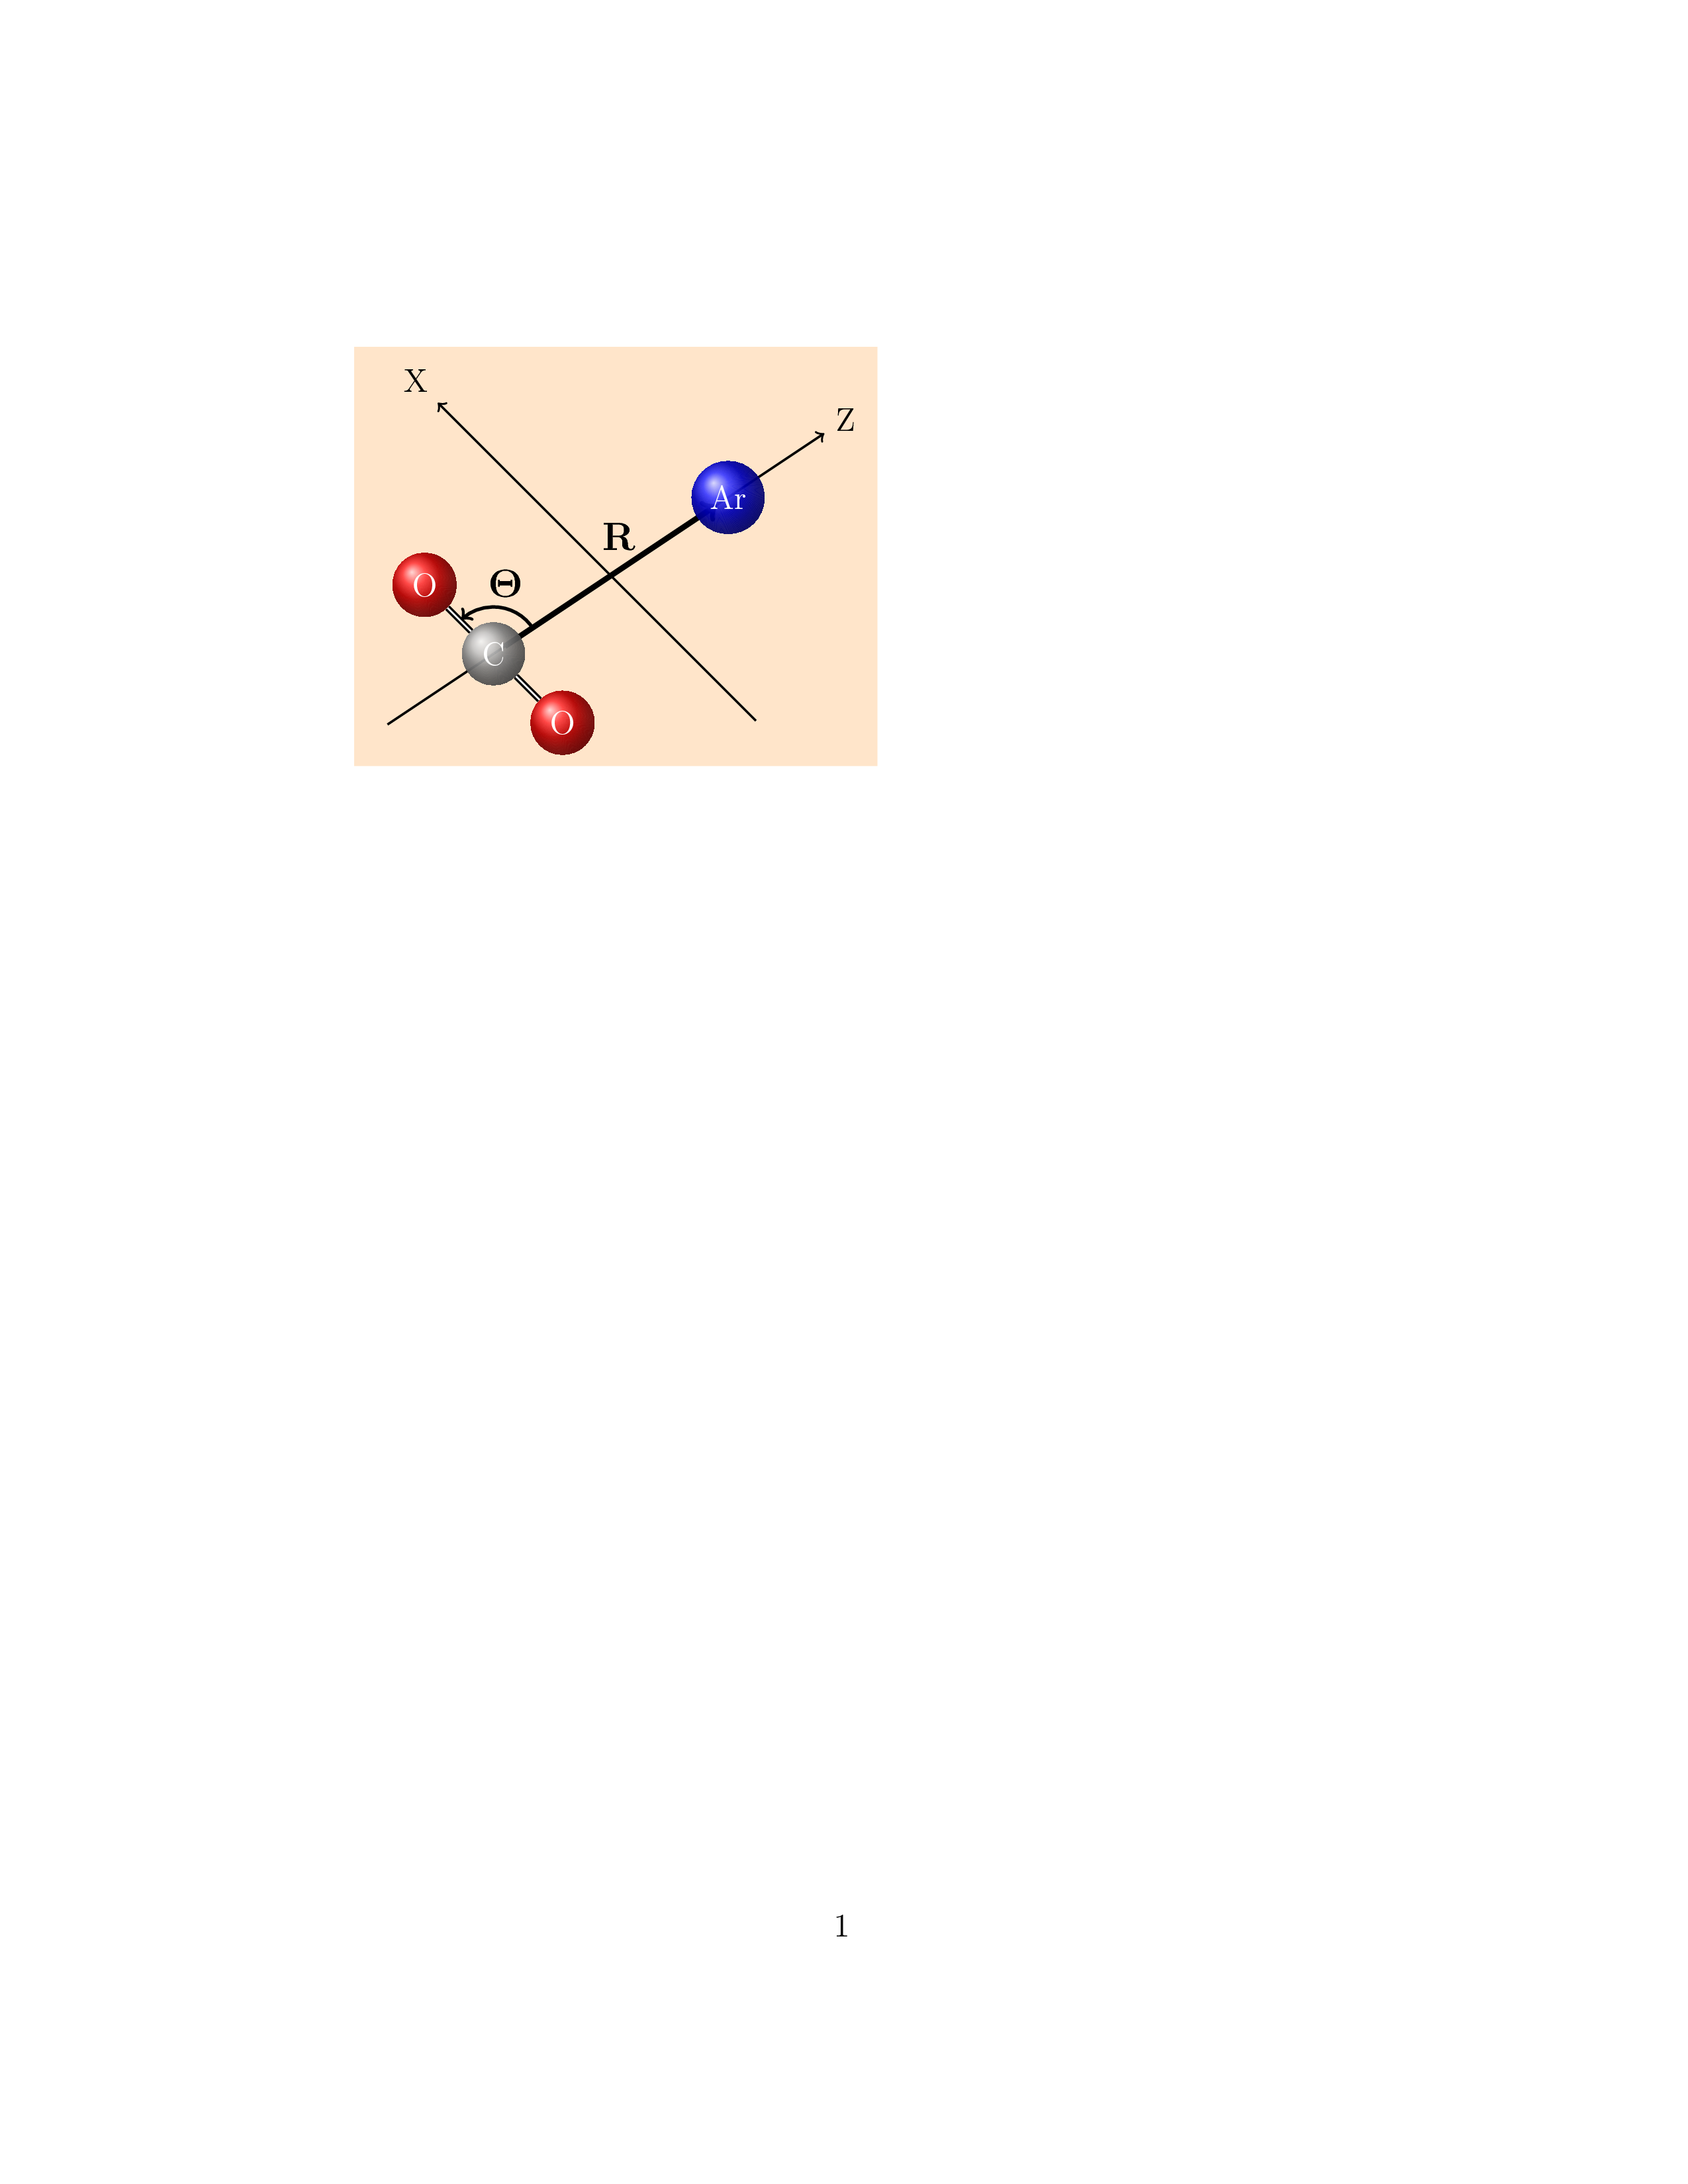
\includegraphics[width=0.5\textwidth]{../pictures/coordsys/coordsys.png}
		%\end{tikzfigure}
}

\block[titleoffsety=1.5cm, bodyoffsety=1.5cm]{Conclusion}{
		The results reported in the present paper demonstrate capability of classical methods to characterize collision-induced absorption in the far-infrared spectral range with an accuracy comparable with THAT EXPERIMENTAL. No use of adjustable parameters is required provided potential energy and induced dipole surfaces are obtained as a result of the high-level \textit{ab initio} calculations and no omission is made in kinetic energy terms of the classical Hamiltonian. The results obtained so far encourage us to extend our approach to other molecular pairs the knowledge of the dipole-forbidden absorption in which is in high demand by the planetary atmospheres investigators.
}

\end{columns}

\end{document}


Classical expressions are obtained for the zeroth and the second spectral moments in which anisotropy of intermolecular interaction is explicitly taken into account for the first time. The comparison of our calculated and available experimental data is discussed for both mixed second virial coefficient and spectral moments of the RT CIA band in $CO_2-Ar$ pairs. \par

